\documentclass[10pt,journal,compsoc]{IEEEtran} %draftclsnofoot, 
\usepackage{graphicx}
\graphicspath{ {./_figures/} }
\setlength\fboxsep{1pt}
\setlength\fboxrule{1pt}
\usepackage{multicol}
\usepackage{bigstrut}
\usepackage{tabularx}
\usepackage{tabulary}
\usepackage{booktabs}
\usepackage{amsmath}
\setlength{\parindent}{0em}
\setlength{\parskip}{1em}
\usepackage{hyperref}
\hypersetup{
  colorlinks = false,
  hidelinks = true
	}
\usepackage[english]{babel}
\usepackage{blindtext}
\usepackage{times}
\usepackage{cite}

\begin{document}
  \markboth{BME 560 Medical Imaging: X-ray, CT, and Nuclear Methods. Fall, 
  2014}%
  {BME 560 Medical Imaging: X-ray, CT, and Nuclear Methods. Fall, 2014}
  
  \title{Intensity Modulated Radiation Therapy using Tomotherapy}
  \author{Rahul Krishna, 
  \IEEEauthorblockA{\normalsize {\textit{Dept. of Electrical and Computer 
  Engineering}\\
    North Carolina State University, Email: 
    \href{mailto:rkrish11@ncsu.edu}{{rkrish11@ncsu.edu}}}}}

	\IEEEcompsoctitleabstractindextext{%
  \begin{abstract}
    Tomotherapy is a form of 3D-conformal radiotherapy which involves the 
    delivery of intensity modulated radiation therapy (IMRT) using rotational 
    fan beam in a manner quite similar to that seen in modern CT scanners. The 
    modern tomotherapy systems have a couch and gantry which are in continuous 
    motion, closely resembeling the traditional helical-CT systems. This kind 
    of radiotherapy is hence called helical tomotherapy. Helical tomotherapy 
    delivers IMRT based on the images of the patient in the treatment position, 
    and these systems do this by acquiring CT images of the patient. This paper 
    is a discourse on the current state-of-the-art in the field, foucsing 
    primarily the technique's conceptual working and results of its clinical 
    implementation. 
    
  \end{abstract}
  % IEEEtran.cls defaults to using nonbold math in the Abstract.
  % This preserves the distinction between vectors and scalars. However,
  % if the journal you are submitting to favors bold math in the abstract,
  % then you can use LaTeX's standard command \boldmath at the very start
  % of the abstract to achieve this. Many IEEE journals frown on math
  % in the abstract anyway. In particular, the Computer Society does
  % not want either math or citations to appear in the abstract.
  
  % Note that keywords are not normally used for peerreview papers.
  \begin{IEEEkeywords}
    Tomotherapy, Intensity Modulated Radiation Therapy.
  \end{IEEEkeywords}}
  \maketitle
  
  \section{Introduction}
	\IEEEPARstart{T}{he} past couple of decades have seen tremendous advances in 
	radiation oncology. The advent of faster and smaller computers has helped 
	transform the field of radiation therapy and treatment planning. The term 
	tomotherapy translates to ``slice therapy'', and it is derived from 
	tomography. Tomotherapy is a form of 3D Conformal Radiotherapy (3D-CRT), 
  which aims to conform the spatial distribution of the prescribed dose to a 
  target volume. The volume includes the cancerous cells plus a margin for 
  spatial uncertainties. While doing do it tries to minimize the dose to the
  surrounding normal structures. The tomotherapy system is designed to make use 
  of the tomographic 	reconstruction mathematics for treatment and also for 
  verification. The idea 	was conceived to tackle several major issues that 
  plagued radiation oncology. One of the primary issues was the limitation of 
  target dose that can be 	delivered due to the presence of neighboring 
  sensitive sturctures. One of the 	potential solutions to avoiding this was 
  to make use of multiple radiation 	beams with non-uniform beam intensities. 
  This method allows one to conform 	the radiation to the target region 
  thereby   sparing the sensitive normal 	structures which would otherwise 
  prevent   normal dose delivery to the affected 	region, see Fig. \ref{intro}.
  
  The setup has a 
  linear accelerator mounted on a rotating gantry as seen in CT 
  sacnners. The radiation is delivered to a patient in a helical way, obtained 
  by concurrent gantry rotation and couch/patient travel as shown in Fig. 
  \ref{fig1}. In general, the helical tomotherapy units have significantly 
  different radiation fields when compared to other radiotherapy systems. This 
  difference can be owed to the absence of absence of a flattening filter, a 
  thin target, an electron stopper, a beam hardener and a compact primary 
  collimator. This paper will briefly highlight the 
  radiation characteristics of the helical tomotherapy unit, especially in 
  parts where it differs from standard accelerators.
  
  The rest of this paper is 
  organized as follows. Section \ref{history} talks 
  about the history of tomotherapy. Section \ref{methods} has 3 subsections: 
  \ref{construction} talks about the construction of the tomotherapy unit, 
  \ref{radiation} discusses the radiation characteristics of helical 
  tomotherapy, and \ref{comparisions} brielfy examines the differences between 
  this techique and other conformal therapy techniques. Section \ref{clinical} 
  is a collection of some clinical results where tomotherapy has been, and has 
  not been, effective. Finally, section \ref{conclusions} presents concluding 
  remarks on the the topic. 
  
   
  \begin{figure}[htbp!]
    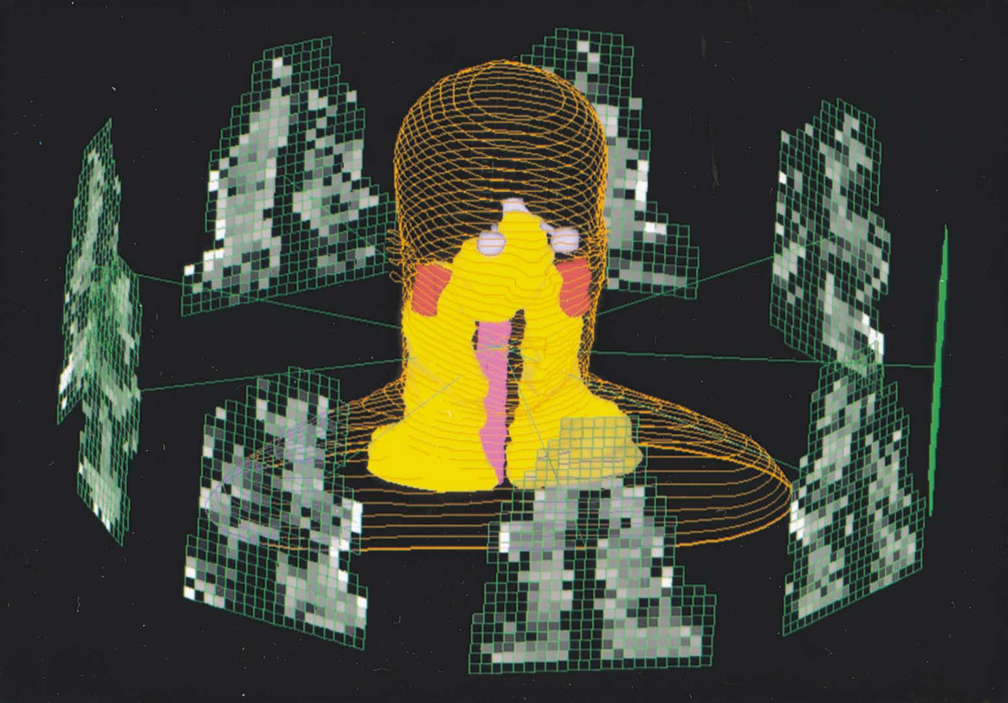
\includegraphics[width=\linewidth]{intro}
    \label{intro}
    \caption{An example of treatment planning in a modern 3D-CRT. In this 
    example, a 3D view of the patient, the PTV, spinal cord, and parotid 
    glands, and the 9 intensity modulated beams used to generate the IMRT dose 
    distribution can be seen. \textit{Image courtesy \cite{IMRT}}}
  \end{figure}
  
  \begin{figure*}[t!]
    \centering
  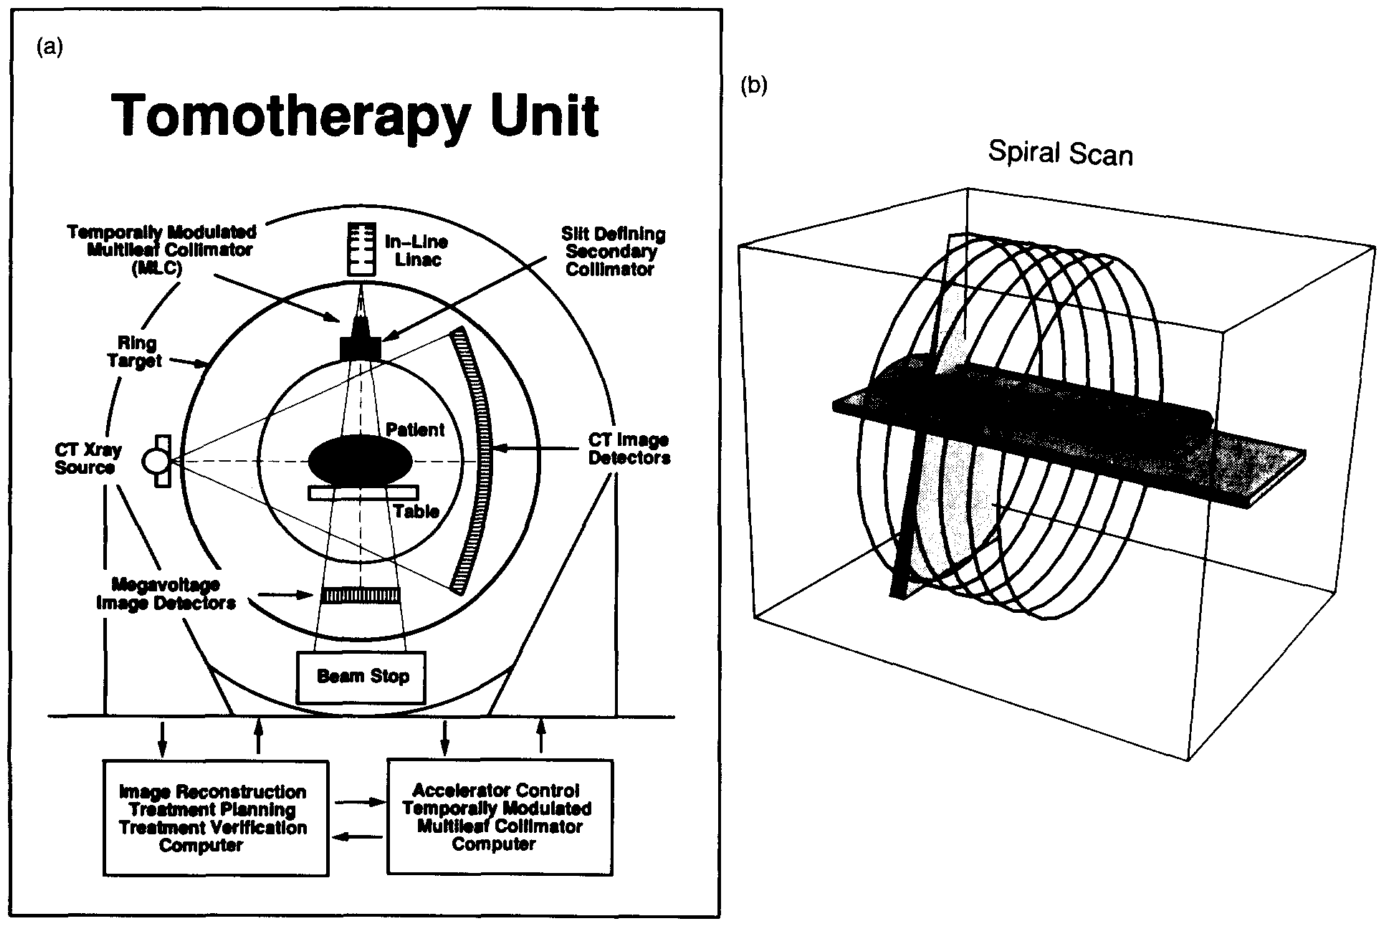
\includegraphics[width=0.9\linewidth]{fig1}
  \caption{A traditional tomotherapy unit, Ref \cite{Mackie1993}. (a) A block 
    diagram showing the ring gantry, and the radiation source}
  \label{fig1}
  
\end{figure*}

\begin{figure}[htbp!]
  \centering
  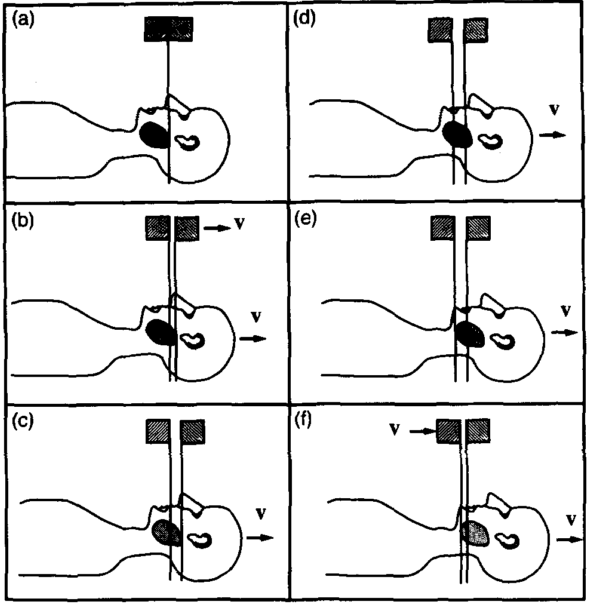
\includegraphics[width=0.921\linewidth]{fig2}
  \caption{``Running start-stop'' mechanism as proposed in Ref. 
    \cite{Mackie1993}. (a)--(c) }
  \label{fig2}
  
\end{figure}
	%----------------------------------
	% References
  %----------------------------------
  \section{History}
  \label{history}
  Tomotherapy was designed in the University of Wisconsin - Madison and 
  TomoTherapy Inc., Madison, WI. The first prototype investigated in this study 
  was installed at University of Wisconsin Hospital and Clinics in Madison, WI, 
  USA. The first paper on tomotherapy was submitted in 1992, Ref. 
  \cite{Mackie1993}. This paper described most of the details seen in the 
  modern sytems used today. This paper also introducted the idea of using a 
  continuously moving slip-ring gantry. The usage of fan-beam to form a 
  modulating beam, and a temorally modulating collimator assembly (this came 
  to be known as the `Binary Collimator') was also initially proposed in this 
  paper. It also recommended performing 
  intensity modulation without the use of a field flattening filter, thus 
  improving the spectrum across the beam.
  
  Several initial theories proposed in the paper could not be implemented. For 
  instance, to address the target cooling issue that is faced in modern photon 
  beam radiotherapy, the authors proposed engineering a stationary ``hoop'' 
  target with water supplied cooling; this could not be implemented due to the 
  increased collimation complexity. Also, in order to give a steep penumbra to 
  the target region, the authors of the original paper proposed a 
  ``start-stop'' mechanism where the collimator jaws defining the slice width 
  would be 
  close and later on as the patient traverses through the field the opposite 
  would happen. Fig. \ref{fig2}, taken from Ref. \cite{Mackie1993}, shows how 
  this was supposed to happen. But, this idea wasn't implementable either, 
  mainly because the technique required the jaws to be in movement during 
  treatment, optimization of beams near the ‘bow’ and the ‘stern’ of the 
  tumour may limit the amount of dose received.
  
  For a more comprehensive history of this form of radiotherapy the readers 
  might want to refer to \cite{Mackie2006}. 
  
  \section{Methods and Materials}
  \label{methods}
  \subsection{Construction}
  \label{construction}
  \subsubsection{A note on Serial Tomotherapy}
  \subsection{Radiation Characteristics}
  \label{radiation}
  \subsection{Comparisions between other conformal therapy techniques}
  \label{comparisions}
    \begin{table*}[htbp]
      \centering
      \caption{A comparision between standard and non-standard IMRT delivery 
      systems (Ref. \cite{Fenwick2006})}
      \small{
      \begin{tabulary}{\linewidth}{LLLLLLL}
        \toprule[0.04cm]
        
        \textbf{System} & \textbf{Gantry} & \textbf{ Beam Geometry} & 
        \textbf{Collimated} & \textbf{Modulated} & \textbf{Imaging} & 
        \textbf{Gating
          Potential} \\\toprule[0.04cm]
        
        Conventional linac plus multileaf & C-Arm & Non-coplanar cone beam & 
        Jaws 
        with conventional
        multileaf & Jaws with conventional
        multileaf & Portal image, fluoroscopy, kvCT, 
        infrared 
        reflectors &
        Breath-hold, 
        beam trigger, multileaf tracking \bigstrut\\\midrule
        Conventional linac minus multileaf & C-Arm & Non-coplanar cone beam & 
        Jaws with/without tertiary attenuator
        & Jaws with/without tertiary attenuator
        & Portal image, fluoroscopy, kvCT, infrared 
        reflectors & Breath-hold,
        beam trigger,
        jaw tracking \bigstrut\\\midrule
        Serial tomotherapy & C-Arm & Fanbeam, coplanar, sequential,
        indexed trajectory & Jaws with binary
        multileaf & Binary multileaf & Portal image, 
        fluoroscopy, kvCT, infrared reflectors & Breath-hold
        during each
        slice \bigstrut\\\midrule
        Helical tomotherapy & Ring  &  Fanbeam,
        coplanar, helical
        trajectory & Jaws with binary
        multileaf & Binary multileaf & MVCT, infrared 
        reflectors & Delivery
        synchronized
        with breathing
        cycle \bigstrut \\\midrule
        Robotic linac & Robotic Arm &  Pencil-beam,
        noncoplanar & Circular collimator & Superposition of pencilbeams by 
        robotic arm & Biplanar radiography, infrared 
        reflectors & Beam 
        trigger,
        robotic
        tracking \bigstrut \\
        \bottomrule
      \end{tabulary}}%
    
      \label{tab:addlabel}%
    \end{table*}%
  \section{Clinical Results}
  \label{clinical}
  \subsection{Total Body Irradiation (TBI)}
  \subsection{Whole brain helical Tomotherapy}
  \subsection{Inoperable Lung Cancer}
  \subsection{Rectal Cancer}
  \section{Conclusion}
  \label{conclusions}
  \bibliography{Paper}{}
  \bibliographystyle{IEEEtran}
  
\end{document}